\chapter{Aplicações a grandes redes e Observações}
De modo a verificar a validade dos nossos algoritmos estes foram aplicados a 
várias redes de testes verificando o tempo de computação e o uso de memória (ver 
tabela~\ref{tbl:tm}) na plataforma Giraph.
\begin{table}
	\centering
 \begin{tabular}{|l|l|l|l|l|l|l|}
 \hline
			Algoritmo & 250k & 500k & 750k & 1000k & Twitter - 1 & Twitter - 2\\ \hline
			Louvain Distribuído&334,4s&589,2s&663s&811s&754s&1737,2s\\ \hline
			Louvain Original&6s&20,4s&41,6s&66,6s&28s&126,3s\\ \hline
			LLP Distribuído& 842s & 1531s & 2372s & 3566s & 1651s &	
1336s
\\ \hline
			LLP Paralelo&24s&59s&116s&187s&14s&36s \\ \hline
		\end{tabular}
		\caption{Esta tabela mostra o desempenho dos nossos algoritmos,
		da implementação original do Louvain 
\textit{Method}~\cite{orgLouvain} e de uma implementação paralela na plataforma 
WebGraph do Layered Label Propagation~\cite{prlLLP}}
		\label{tbl:tm}
\end{table}

  Para os testes da foram geradas redes de diferentes tamanhos sendo todas 
elas densas. Também são usadas duas redes reais resultante de mensagens 
provenientes do Twitter entre utilizadores com 1,33 milhões (Twitter - 1) de nós 
e 3,46 milhões (Twitter - 2) de nós. Em todos os casos foi observado um maior 
tempo de computação nas nossas versões distribuídas dos algoritmos.

Testes do Louvain Distribuído mostraram que a opção de modularidade mínima 
permitida varia o tempo de computação até um valor máximo onde este estabiliza, 
faltando testar a qualidade das comunidades geradas com diversos valores de 
modularidade mínima. 
Sendo que a modularidade mínima permitida modifica as mudanças de comunidade
por cada nó foi também observado este pode levar a poucas ou nenhuma mudanças 
quando maior ou igual que um certo valor. Sendo este valor 1 para as redes 
densas testados mas as redes do Twitter sendo esparsas, mostram responder melhor 
a valores superior a 1. Valores muito pequenos levaram a diversas mudanças e por 
isso, um grande tempo de computação.

Para os testes entre a versão do \textit{Layered Label Propagation} distribuído 
foi utilizado o algoritmo \ref{llpdistributed2}. Devido à inexistência de um 
ambiente que tivesse as especificações perto do distribuído, os testes do 
\textit{Layered Label Propagation} paralelo foram executados numa das maquinas 
que constituí o ambiente distribuído, sendo esta máquina \textit{singlecore}.

Foi também feito testes de escalabilidade executando os algoritmos com um número diferente de máquinas, sendo os resultados presentes nas imagens~\ref{louvainesc} e~\ref{llpesc}.

\begin{figure}
  \centering
  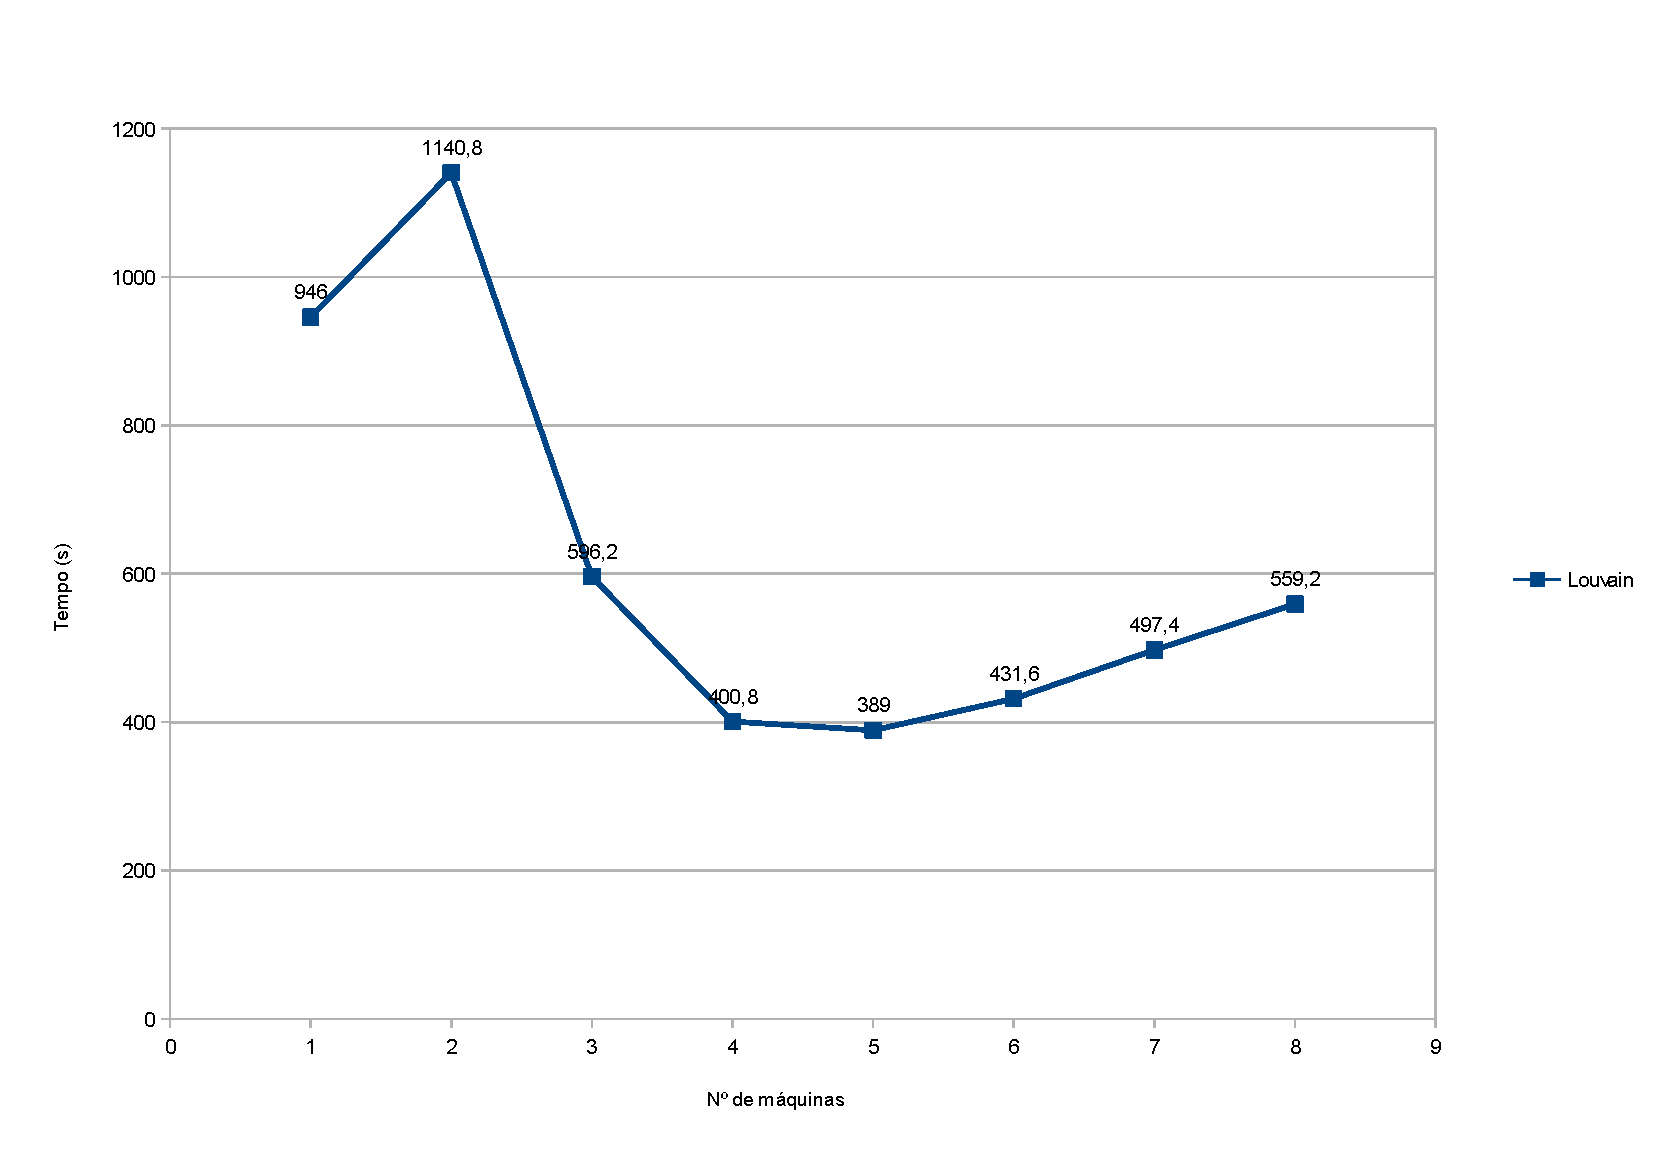
\includegraphics[width=\linewidth]{lov}
  \caption{Testes de escalabilidade usando o algoritmo de Louvain Method. Foi usado um grafo de 500 mil vértices, variando o número de máquinas intervenientes.}
	\label{louvainesc}
\end{figure}

Em ambos os casos foram observados tempos de computação menores quando são usadas quatro e cinco máquinas e maiores quando perto de duas. Depois de duas máquinas o tempo de computação parece diminuir rapidamente até a um certo até ponto e dai tem aumentos.

\chapter{Conclusão}
Foi criada uma biblioteca que uniformiza o desenvolvimento para as duas bibliotecas BSP Apache Giraph e Apache Hama permitindo que se desenvolva código para ambas apenas uma vez. O outro alvo deste trabalho, o desenvolvimento de vários algoritmos que permitem análise a redes de grande dimensão, foi também concluído e foram feitas análises a estes em comparações a outros algoritmos existentes, nomeadamente, versões não distribuídas dos tais.

A biblioteca foi feita de modo a que o mínimo trabalho seja necessário para executar algoritmos nas duas bibliotecas deixando a possibilidade de introduzir compatibilidade com outra biblioteca que siga o mesmo modelo. Os algoritmos que foram implementados sobre esta biblioteca são algoritmos que permitem efetuar diversos tipos de análises a redes de grande dimensão permitindo que alguém utilize esta biblioteca para este feito sem ter necessidade de implementar novos algoritmos.

É possível concluir com estas análises que as versões não distribuídas têm uma vantagem em termos de tempos de computação mas graças ao modelo distribuído dos nossos algoritmos é estimado que os nossos algoritmos possam ser executados sobre redes de dimensões maiores que as versões não distribuídas pois estas deparam-se eventualmente com o \textit{bottleneck} do custo de memória mais rapidamente que o nosso.

Nos testes de escalabilidade é possível ver que o tempo de computação varia com um número de máquinas usadas para computação existindo um número de máquinas ideal para a execução dos algoritmos. As diferenças nos tempos pode ser devido ao \textit{overhead} causado pela comunicação entre as várias máquinas o que explicaria o resultado de usar uma só máquina ser melhor do que usar duas. É esperado que o número ideal de máquinas varie com o tamanho da rede e que após um certo tamanho o \textsl{overhead} seja desprezável.

